\documentclass[aspectratio=169,11pt]{beamer}

\usetheme{Madrid}
\usecolortheme{default}
\setbeamertemplate{navigation symbols}{}
\setbeamertemplate{footline}[frame number]

\usepackage{booktabs}
\usepackage{amsmath,amssymb}
\usepackage{graphicx}
\usepackage{hyperref}
\usepackage{tikz}
\usetikzlibrary{arrows.meta,positioning,fit,calc}

\title{Weak Endogenous NEAT:\\Experiments and Results}
\subtitle{Setup, terminology, and comparison of modes}
\author{Endogenous-Parameter NEAT prototype}
\date{\today}

\begin{document}

\begin{frame}
  \titlepage
\end{frame}

\begin{frame}{Outline}
  \tableofcontents
\end{frame}

%----------------------------------------------------------------------
\section{Motivation and terminology}
%----------------------------------------------------------------------

\begin{frame}{Classical NEAT in one slide}
  \textbf{NEAT} (NeuroEvolution of Augmenting Topologies) evolves neural networks by
  mutating \emph{topology} and \emph{weights}.

  \vspace{0.8em}
  Classical description:
  \[
    G_t = (A_t,\, w_t),\qquad
    G_{t+1} = M_{\mathrm{NEAT}}(G_t;\,\lambda)
  \]
  \begin{itemize}
    \item $A_t$: network topology (nodes and connections)
    \item $w_t$: connection weights (and related gene attributes)
    \item $\lambda$: \textbf{fixed} mutation-control parameters set by the experimenter
      (in a config file)
  \end{itemize}

  \vspace{0.5em}
  Examples of $\lambda$: probability of adding a node, rate/power of weight mutation, \ldots
\end{frame}

\begin{frame}{What is $\theta$ (theta)?}
  In this project, \textbf{$\theta$} is a vector of \emph{per-genome}
  mutation-control parameters---the endogenous analogue of $\lambda$.

  \vspace{0.6em}
  Weak endogenous NEAT:
  \[
    G_t = (A_t,\, w_t,\, \theta_t),\qquad
    G_{t+1} = M_{\mathrm{NEAT}}(G_t;\,\theta_t)
  \]

  \begin{block}{Properties of $\theta$}
    \begin{itemize}
      \item Encoded in each genome (not only in the global config)
      \item Inherited at crossover
      \item Mutated slightly between generations
      \item Optionally rewritten by network \textbf{meta-outputs} (\texttt{meta-theta} mode)
      \item Always clipped to fixed bounds
    \end{itemize}
  \end{block}
\end{frame}

\begin{frame}{The eight components of $\theta$}
  \begin{tabular}{lll}
    \toprule
    Field & Role & Typical bounds \\
    \midrule
    \texttt{node\_add\_prob} & $P$(add hidden node) & $[0,\,0.5]$ \\
    \texttt{node\_delete\_prob} & $P$(delete node) & $[0,\,0.5]$ \\
    \texttt{conn\_add\_prob} & $P$(add connection) & $[0,\,0.8]$ \\
    \texttt{conn\_delete\_prob} & $P$(delete connection) & $[0,\,0.8]$ \\
    \texttt{weight\_mutate\_rate} & $P$(mutate a weight) & $[0,\,1]$ \\
    \texttt{weight\_mutate\_power} & size of weight noise & $[0.001,\,5]$ \\
    \texttt{bias\_mutate\_rate} & $P$(mutate a bias) & $[0,\,1]$ \\
    \texttt{enable\_disable\_rate} & $P$(toggle connection) & $[0,\,0.5]$ \\
    \bottomrule
  \end{tabular}

  \vspace{0.8em}
  Defaults match the NEAT config (e.g.\ weight mutate rate $0.8$, power $0.5$).
\end{frame}

\begin{frame}{Important claim: \emph{weak} endogeneity}
  \begin{alertblock}{What we claim}
    Selected \textbf{operator-control parameters} are in the genome, inherited, mutated,
    selected, and (in one mode) modified by network meta-outputs.
  \end{alertblock}

  \begin{block}{What we do \emph{not} claim}
    \begin{itemize}
      \item Fully self-replicating neural networks
      \item The network implements its own reproduction algorithm
      \item Complete endogenous evolution
    \end{itemize}
  \end{block}

  Reproduction (selection, crossover, speciation) remains an \textbf{external}
  NEAT implementation (\texttt{neat-python}).
\end{frame}

\begin{frame}{Glossary}
  \begin{description}
    \item[$\lambda$] Global mutation parameters in the config (classical NEAT).
    \item[$\theta$] Per-genome mutation parameters (this prototype).
    \item[Task output] Network output used for fitness (always \texttt{output[0]}).
    \item[Meta-outputs] Extra outputs \texttt{output[1..8]} that can set $\theta$.
    \item[$\theta$ inputs] Current $\theta$, unit-normalized, concatenated to task state.
    \item[Network rewrite] In \texttt{meta-theta}: replace $\theta$ after eval from
      averaged meta-outputs (full replacement, not a blend); next eval sees new $\theta$ inputs.
    \item[Matched capacity] All modes use the same I/O sizes (fair comparison).
    \item[Solve] Best fitness reaches a task-specific threshold.
    \item[Generation] One evaluate $\rightarrow$ reproduce cycle.
    \item[Run] One independent evolution (own random seed / trajectory).
  \end{description}
\end{frame}

%----------------------------------------------------------------------
\section{Experimental setup}
%----------------------------------------------------------------------

\begin{frame}{Software stack}
  \begin{itemize}
    \item Base library: local fork of \textbf{neat-python} (submodule)
    \item Prototype package: \texttt{endogenous\_neat}
    \item Extensions:
      \begin{itemize}
        \item \texttt{Theta} dataclass
        \item \texttt{EndogenousGenome} (extends \texttt{DefaultGenome})
        \item \texttt{EndogenousReproduction} (thin wrapper)
      \end{itemize}
    \item CLI: \texttt{python -m endogenous\_neat.experiment --task \ldots\ --mode \ldots}
  \end{itemize}
\end{frame}

\begin{frame}{Three comparison modes}
  \begin{center}
  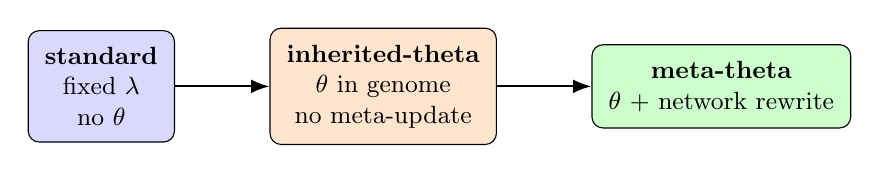
\begin{tikzpicture}[
    box/.style={draw,rounded corners,align=center,inner sep=6pt,font=\small},
    arr/.style={-{Latex},thick}
  ]
    \node[box,fill=blue!15] (std) {\textbf{standard}\\fixed $\lambda$\\no $\theta$};
    \node[box,fill=orange!20,right=1.2cm of std] (inh)
      {\textbf{inherited-theta}\\$\theta$ in genome\\no meta-update};
    \node[box,fill=green!20,right=1.2cm of inh] (meta)
      {\textbf{meta-theta}\\$\theta$ + network rewrite};
    \draw[arr] (std) -- (inh);
    \draw[arr] (inh) -- (meta);
  \end{tikzpicture}
  \end{center}

  \vspace{0.8em}
  \begin{itemize}
    \item \textbf{standard}: classical NEAT; mutation rates from config only
    \item \textbf{inherited-theta}: $\theta$ inherited \& randomly mutated; network does not write $\theta$
    \item \textbf{meta-theta}: after evaluation, replace $\theta$ from meta-outputs
  \end{itemize}
\end{frame}

\begin{frame}{How $\theta$ is used at mutation time}
  For endogenous genomes, mutation does \emph{not} permanently overwrite the shared config.

  \vspace{0.5em}
  \begin{enumerate}
    \item Build a local copy of the genome config
    \item Overlay this genome's $\theta$ onto mutation rates
    \item Call standard NEAT \texttt{mutate} with that local config
    \item Apply a small random mutation to $\theta$ itself
  \end{enumerate}

  \vspace{0.5em}
  Speciation distance also includes a small $\theta$ term
  (coefficient $0.1$ times $L_1$ distance of $\theta$ vectors).
\end{frame}

\begin{frame}{Network rewrite in \texttt{meta-theta}}
  \textbf{Network rewrite} $=$ after evaluating a genome, its $\theta$ is
  \emph{discarded and replaced} by values computed from the network's extra outputs.

  \vspace{0.6em}
  Place in the generation loop:
  \begin{enumerate}
    \item Build network from genome
    \item Activate with task state $+$ \emph{current} normalized $\theta$
    \item Fitness $\leftarrow$ \texttt{out}$_0$ only
    \item Meta-outputs $\leftarrow$ average of \texttt{out}$_{1..8}$ over the evaluation
    \item \alert{\texttt{genome.theta} $\leftarrow$ \texttt{Theta.from\_meta\_outputs(mean\_meta)}}
    \item Later activates / next generation use the updated $\theta$ as inputs
  \end{enumerate}

  \vspace{0.4em}
  Step~5 is the rewrite. In \texttt{inherited-theta}, step~5 is skipped
  (but $\theta$ inputs still track the inherited/mutated genome $\theta$).
\end{frame}

\begin{frame}{What the network outputs mean}
  All modes use \textbf{9 outputs}; only \texttt{meta-theta} uses heads $1$--$8$ for $\theta$:

  \vspace{0.4em}
  \begin{tabular}{cl}
    \toprule
    Output & Role \\
    \midrule
    \texttt{out}$_0$ & Task (XOR answer or pole force) \\
    \texttt{out}$_1$ & $\rightarrow$ \texttt{node\_add\_prob} \\
    \texttt{out}$_2$ & $\rightarrow$ \texttt{node\_delete\_prob} \\
    \texttt{out}$_3$ & $\rightarrow$ \texttt{conn\_add\_prob} \\
    \texttt{out}$_4$ & $\rightarrow$ \texttt{conn\_delete\_prob} \\
    \texttt{out}$_5$ & $\rightarrow$ \texttt{weight\_mutate\_rate} \\
    \texttt{out}$_6$ & $\rightarrow$ \texttt{weight\_mutate\_power} \\
    \texttt{out}$_7$ & $\rightarrow$ \texttt{bias\_mutate\_rate} \\
    \texttt{out}$_8$ & $\rightarrow$ \texttt{enable\_disable\_rate} \\
    \bottomrule
  \end{tabular}
\end{frame}

\begin{frame}{Averaging before the rewrite}
  Meta heads can change on every activation, so they are averaged
  \textbf{once per genome} after evaluation:

  \vspace{0.5em}
  \begin{itemize}
    \item \textbf{XOR:} mean of \texttt{out}$_{1..8}$ over the 4 input cases
    \item \textbf{Pole:} mean of \texttt{out}$_{1..8}$ over all timesteps of all episode runs
  \end{itemize}

  \vspace{0.5em}
  Result: one length-$8$ vector \texttt{mean\_meta}.
  This avoids updating $\theta$ after every single activation in an order-dependent way.
\end{frame}

\begin{frame}{Mapping meta-outputs $\rightarrow$ $\theta$}
  Meta-heads already use neat-python's sigmoid, so $x_i\in(0,1)$.
  Do \emph{not} apply a second sigmoid (that would squash into $\sim[0.5,0.73]$
  and push $\theta$ into the upper half of each bound).
  Map linearly into the legal range $[m_i,M_i]$:
  \[
    \theta_i = m_i + \mathrm{clamp}(x_i,0,1)\,(M_i - m_i)
  \]

  \vspace{0.4em}
  \begin{itemize}
    \item $x \approx 0$ $\rightarrow$ near minimum
    \item $x \approx 0.5$ $\rightarrow$ mid-range of the bound
    \item $x \approx 1$ $\rightarrow$ near maximum
  \end{itemize}

  \vspace{0.4em}
  Then: \texttt{genome.theta = Theta.from\_meta\_outputs(mean\_meta)}\\
  --- still a \textbf{full replacement}, not a blend with the old $\theta$
  (no residual / $\alpha$-update yet).

  \vspace{0.4em}
  \begin{alertblock}{Earlier bug}
    First experiments used a \emph{second} sigmoid on already-sigmoid outputs
    (``double sigmoid'') $\Rightarrow$ systematically aggressive $\theta$.
  \end{alertblock}
\end{frame}

\begin{frame}{Speciation note (matched 9-output nets)}
  With $\theta$ inputs and a small $\theta$ distance term, genomic distances inflate.
  Too low a threshold creates more species than
  \texttt{pop\_size} / \texttt{min\_species\_size} allows
  (neat-python then aborts during spawn adjustment).

  \vspace{0.6em}
  Current configs use \texttt{compatibility\_threshold}${}=10.0$
  (XOR pop.\ $150$, pole pop.\ $250$).
\end{frame}

\begin{frame}{What network rewrite is \emph{not}}
  \begin{itemize}
    \item It does \textbf{not} change network weights or topology at evaluation time
    \item It does \textbf{not} change how fitness is computed (still only \texttt{out}$_0$)
    \item It only changes the genome's \textbf{mutation-control vector} $\theta$
      used in the \textbf{next} reproduction step
  \end{itemize}

  \vspace{0.6em}
  \begin{alertblock}{Consequence}
    $\theta$ inherited from parents can be overwritten every generation.
    If meta-heads saturate, $\theta$ jumps toward extreme bounds
    (e.g.\ high \texttt{weight\_mutate\_power}) even when that hurts the task.
  \end{alertblock}
\end{frame}

\begin{frame}{Matched topology capacity}
  To compare modes fairly, \textbf{all modes} use the same network I/O layout:

  \begin{itemize}
    \item XOR: \textbf{10 inputs} (2 task + 8 $\theta$), \textbf{9 outputs}
    \item Pole: \textbf{12 inputs} (4 task + 8 $\theta$), \textbf{9 outputs}
  \end{itemize}

  \vspace{0.5em}
  Layout:
  \[
    \underbrace{\text{task state}}_{\text{XOR / pole}} \;+\;
    \underbrace{\hat\theta_{1..8}}_{\text{normalized current $\theta$}}
    \;\rightarrow\;
    \underbrace{\texttt{out}_0}_{\text{task}} \;+\;
    \underbrace{\texttt{out}_{1..8}}_{\text{meta / $\theta$}}
  \]

  \begin{itemize}
    \item Fitness always uses \texttt{out}$_0$ only
    \item $\theta$ inputs are unit-normalized from current \texttt{genome.theta}
      (defaults in \texttt{standard})
    \item After a meta rewrite, the next evaluation feeds the updated $\theta$
    \item In \texttt{standard} / \texttt{inherited-theta}, meta heads exist but are ignored
  \end{itemize}
\end{frame}

%----------------------------------------------------------------------
\section{Tasks}
%----------------------------------------------------------------------

\begin{frame}{Task 1: XOR (10-in / 9-out)}
  Classic Boolean XOR, but with matched $\theta$ inputs and 9 network outputs.

  \vspace{0.5em}
  \begin{columns}[t]
    \begin{column}{0.48\textwidth}
      \textbf{Inputs / targets}
      \begin{center}
      \begin{tabular}{cc}
        \toprule
        Input & Target \\
        \midrule
        $(0,0)$ & $0$ \\
        $(0,1)$ & $1$ \\
        $(1,0)$ & $1$ \\
        $(1,1)$ & $0$ \\
        \bottomrule
      \end{tabular}
      \end{center}
      plus 8 normalized $\theta$ channels
    \end{column}
    \begin{column}{0.48\textwidth}
      \textbf{Fitness}
      \[
        F = 4 - \sum (\hat y - y)^2
      \]
      \textbf{Solved} if $F \ge 3.9$

      \vspace{0.6em}
      Population size $150$\\
      Fitness plateau $F\approx 3.0$
      $\Leftrightarrow$ constant $\sim 0.5$ outputs
    \end{column}
  \end{columns}
\end{frame}

\begin{frame}{Task 2: Single-pole balancing}
  Cart--pole control (feedforward), adapted from neat-python examples.

  \vspace{0.5em}
  \begin{itemize}
    \item \textbf{State}: 4 scaled cart-pole channels \textbf{+} 8 normalized $\theta$
      (12 inputs total)
    \item \textbf{Action}: discrete force from \texttt{out}$_0$ ($+10$ or $-10$)
    \item \textbf{Fitness}: worst balance time (seconds) over 5 random starts, cap $60\,\mathrm{s}$
    \item \textbf{Solved} if $F \ge 60.0$
    \item Population size $250$
  \end{itemize}

  \vspace{0.5em}
  Again: 9 outputs total (1 control + 8 meta) in all modes.
\end{frame}

\begin{frame}{What we measure}
  Per run (CSV + plots):
  \begin{itemize}
    \item Best / mean fitness vs generation
    \item Best-genome $\theta$ vs generation (endogenous modes)
    \item Population mean / std of $\theta$
  \end{itemize}

  \vspace{0.5em}
  Across modes (\texttt{--mode compare}):
  \begin{itemize}
    \item Solve rate (fraction of runs reaching threshold)
    \item Final best fitness (mean $\pm$ std, median)
    \item Median first-solve generation (among successful runs)
    \item Overlay plots of median fitness $\pm$ IQR and $\theta$ trajectories
  \end{itemize}
\end{frame}

\begin{frame}{Reading the plots carefully}
  \begin{alertblock}{Early stopping}
    When fitness hits the threshold, evolution stops.
    Median fitness curves for successful modes look ``short''---that means
    \textbf{solved}, not crashed.
  \end{alertblock}

  \begin{itemize}
    \item Prefer \textbf{solve rate} and \textbf{time-to-threshold} over truncated median curves
    \item Median fitness stays near a plateau until $>$ half of runs escape it
    \item Mixing short smoke tests with long runs in one folder corrupts comparisons
  \end{itemize}
\end{frame}

%----------------------------------------------------------------------
\section{Results}
%----------------------------------------------------------------------

\begin{frame}{Two mapping regimes}
  Results below distinguish:

  \vspace{0.5em}
  \begin{description}
    \item[Double sigmoid] Early Phase~1: $\theta_i = m_i + \sigma(x_i)(M_i-m_i)$
      on already-sigmoid $x_i$ (biased toward upper half of bounds).
    \item[Linear map] Current code: $\theta_i = m_i + \mathrm{clamp}(x_i,0,1)(M_i-m_i)$.
  \end{description}

  \vspace{0.6em}
  Full $\theta$ replacement each generation is unchanged in both regimes.
\end{frame}

\begin{frame}{Third change: $\theta$ as network inputs}
  After linear mapping, we added \textbf{8 normalized $\theta$ channels} to the
  network input vector (all modes, matched capacity):

  \vspace{0.5em}
  \begin{itemize}
    \item XOR: $2$ task bits $+$ $8\,\hat\theta$ $\rightarrow$ \textbf{10 inputs}
    \item Pole: $4$ state channels $+$ $8\,\hat\theta$ $\rightarrow$ \textbf{12 inputs}
    \item Endogenous modes: inputs track live \texttt{genome.theta}
    \item \texttt{standard}: inputs use fixed default $\theta$ (same topology)
    \item After meta rewrite: next evaluation uses updated $\theta$ inputs
  \end{itemize}

  \vspace{0.6em}
  Runs: \texttt{xor\_theta\_inputs}, \texttt{pole\_theta\_inputs}\\
  (linear map; \texttt{compatibility\_threshold} raised to $10.0$ during tuning)
\end{frame}

\begin{frame}{XOR (double sigmoid): \texttt{compare\_200x50}}
  Setup: \textbf{50 runs} $\times$ up to \textbf{200 generations} $\times$ 3 modes\\
  (matched 9-output XOR; double-sigmoid meta map)

  \vspace{0.6em}
  \begin{tabular}{lrrr}
    \toprule
    Mode & Solved & Solve rate & Median first solve \\
    \midrule
    standard & $32/50$ & \textbf{64\%} & gen $125$ \\
    inherited-theta & $19/50$ & 38\% & gen $140$ \\
    meta-theta & $2/50$ & 4\% & gen $164$ \\
    \bottomrule
  \end{tabular}

  \vspace{0.8em}
  Ranking: \textbf{standard $\gg$ inherited-theta $\gg$ meta-theta}
\end{frame}

\begin{frame}{XOR (linear map): \texttt{xor\_compare\_linear-3}}
  Setup: \textbf{10 runs} $\times$ up to \textbf{100 generations}; linear meta map;
  \texttt{compatibility\_threshold}${}=4.0$ (pre--$\theta$-input configs)

  \vspace{0.6em}
  \begin{tabular}{lrrr}
    \toprule
    Mode & Solved & Solve rate & Median first solve \\
    \midrule
    standard & $1/10$ & 10\% & gen $73$ \\
    inherited-theta & $0/10$ & 0\% & --- \\
    meta-theta & $0/10$ & 0\% & --- \\
    \bottomrule
  \end{tabular}

  \vspace{0.6em}
  \begin{itemize}
    \item All modes sit on the $F\approx 3.0$ plateau (median curves flat)
    \item Linear map alone does \textbf{not} rescue meta-$\theta$ on XOR
    \item Underpowered vs $200\times 50$; also stricter speciation than the older run
  \end{itemize}
\end{frame}

\begin{frame}{XOR: interpretation}
  \begin{itemize}
    \item Fitness $\approx 3.0$ is a common local plateau (constant mid-outputs)
    \item Under double sigmoid, encoding $\theta$ alone hurts vs fixed $\lambda$
      ($-26$~pp); meta hurts much more ($-60$~pp)
    \item Under linear map (short budget), meta still fails; $\theta$ still
      bound-bangs (\texttt{weight\_mutate\_power} median $\sim 3.4$)
    \item Inherited $\theta$ stays near defaults but does not escape the plateau
      in $100$ gens $\times$ $10$ seeds
  \end{itemize}

  \vspace{0.4em}
  Fair large re-run ($200$ gens, $\ge 30$--$50$ seeds) still needed for the linear map.
\end{frame}

\begin{frame}{Pole (double sigmoid): \texttt{pole\_compare2}}
  Setup: up to \textbf{200 generations}; uneven $n$ (20 / 10 / 10)

  \vspace{0.6em}
  \begin{tabular}{lrrr}
    \toprule
    Mode & Solved & Solve rate & Median first solve \\
    \midrule
    standard & $20/20$ & \textbf{100\%} & gen $22.5$ \\
    inherited-theta & $10/10$ & \textbf{100\%} & gen $15$ \\
    meta-theta & $0/10$ & 0\% & --- \\
    \bottomrule
  \end{tabular}

  \vspace{0.6em}
  Meta-theta finals: median $\approx 9.3\,\mathrm{s}$, mean $\approx 14.7\,\mathrm{s}$
  (best unfinished run $\approx 57.5\,\mathrm{s}$).
\end{frame}

\begin{frame}{Pole (linear map): \texttt{pole\_compare\_linear-2}}
  Setup: \textbf{10 runs}/mode $\times$ up to \textbf{200 generations}; linear meta map

  \vspace{0.6em}
  \begin{tabular}{lrrr}
    \toprule
    Mode & Solved & Solve rate & Median first solve \\
    \midrule
    standard & $10/10$ & \textbf{100\%} & gen $20$ \\
    inherited-theta & $10/10$ & \textbf{100\%} & gen $11$ \\
    meta-theta & $7/10$ & 70\% & gen $23$ \\
    \bottomrule
  \end{tabular}

  \vspace{0.6em}
  \begin{itemize}
    \item Meta solve rate: $0\%$ $\rightarrow$ \textbf{70\%} after removing double sigmoid
    \item Inherited remains fastest to threshold
    \item Three meta failures stay $\sim 2\,\mathrm{s}$ for all $200$ gens
      (final \texttt{weight\_mutate\_power}${}\approx 5$)
  \end{itemize}
\end{frame}

\begin{frame}{XOR ($\theta$ inputs): \texttt{xor\_theta\_inputs}}
  Setup: \textbf{10 runs}/mode $\times$ \textbf{100 generations}; linear map;
  \textbf{10 inputs} ($2$ XOR $+$ $8\,\hat\theta$); \texttt{compat}${}=10.0$

  \vspace{0.6em}
  \begin{tabular}{lrrr}
    \toprule
    Mode & Solved & Solve rate & Median first solve \\
    \midrule
    standard & $0/10$ & 0\% & --- \\
    inherited-theta & $0/10$ & 0\% & --- \\
    meta-theta & $0/10$ & 0\% & --- \\
    \bottomrule
  \end{tabular}

  \vspace{0.6em}
  \begin{itemize}
    \item All modes stuck at $F=3.0$ for all $100$ generations (no run $>3.0$)
    \item Worse than \texttt{xor\_compare\_linear-3} (standard $1/10$ solved)
    \item Meta final $\theta$: \texttt{weight\_mutate\_power} median $\approx 5.0$,
      \texttt{enable\_disable\_rate} $\approx 0.25$
  \end{itemize}
\end{frame}

\begin{frame}{Pole ($\theta$ inputs): \texttt{pole\_theta\_inputs}}
  Setup: up to \textbf{200 generations}; \textbf{12 inputs} ($4$ state $+$ $8\,\hat\theta$);
  \texttt{compat}${}=10.0$; folder merges two compare batches ($n$ uneven for meta)

  \vspace{0.6em}
  \begin{tabular}{lrrr}
    \toprule
    Mode & Solved & Solve rate & Median first solve \\
    \midrule
    standard & $20/20$ & \textbf{100\%} & gen $8$ \\
    inherited-theta & $20/20$ & \textbf{100\%} & gen $12.5$ \\
    meta-theta & $13/18$ & 72\% & gen $54$ \\
    \bottomrule
  \end{tabular}

  \vspace{0.6em}
  \begin{itemize}
    \item Standard / inherited \textbf{faster} than pre-input \texttt{pole\_compare\_linear-2}
      (median gen $20$ / $11$)
    \item Meta solve rate similar ($72\%$ vs $70\%$) but \textbf{slower} when it works
      (median gen $54$ vs $23$)
    \item Second batch alone: meta $10/10$; first batch: meta $3/8$ (speciation crashes)
  \end{itemize}
\end{frame}

\begin{frame}{$\theta$ inputs: interpretation}
  \begin{columns}[t]
    \begin{column}{0.48\textwidth}
      \textbf{Pole}
      \begin{itemize}
        \item Feeding $\hat\theta$ did not break control
        \item Classical / inherited solve \textbf{100\%}, often \textbf{faster}
        \item Meta still fails $\sim 28\%$ of runs
        \item Failures: \texttt{weight\_mutate\_power}${}\approx 5$\\
          Successes: often \emph{low} power ($\sim 0$)
      \end{itemize}
    \end{column}
    \begin{column}{0.48\textwidth}
      \textbf{XOR}
      \begin{itemize}
        \item $\theta$ awareness did \textbf{not} escape $F=3.0$ plateau
        \item Extra inputs + higher speciation pressure may hurt search
        \item Meta still bound-bangs mutation rates
        \item Needs larger budget ($200$ gens, more seeds)
      \end{itemize}
    \end{column}
  \end{columns}

  \vspace{0.8em}
  \begin{block}{Net effect}
    $\theta$ inputs help pole meta \emph{condition} on operator state but do not fix
    XOR; meta-$\theta$ remains a bifurcation (mild $\theta$ vs saturated $\theta$).
  \end{block}
\end{frame}

\begin{frame}{Pole: interpretation}
  \begin{itemize}
    \item Cart-pole is much easier for classical NEAT than 9-output XOR
    \item \texttt{inherited-theta} is \textbf{competitive} (100\%; often faster)
    \item Linear meta map is a \textbf{real improvement} on pole, but not a full fix
    \item Failed meta runs still look like over-aggressive mutation attractors
    \item Overlay fitness/$\theta$ PNGs truncate due to early stopping---prefer solve rates
  \end{itemize}
\end{frame}

\begin{frame}{Cross-task summary}
  \small
  \begin{center}
  \begin{tabular}{lccc}
    \toprule
    Setting & XOR solve (meta) & Pole solve (meta) & Notes \\
    \midrule
    Double $\sigma$, no $\hat\theta$ in & $2/50$ (4\%) & $0/10$ (0\%) & early Phase~1 \\
    Linear map, no $\hat\theta$ in & $0/10$ & $7/10$ (70\%) & \texttt{*\_linear-2/3} \\
    Linear map + $\hat\theta$ in & $0/10$ & $13/18$ (72\%) & \texttt{*\_theta\_inputs} \\
    \midrule
    standard (best pole) & --- & $20/20$ (100\%) & med.\ solve gen $8$ \\
    inherited (best pole) & --- & $20/20$ (100\%) & med.\ solve gen $12.5$ \\
    \bottomrule
  \end{tabular}
  \end{center}

  \vspace{0.6em}
  \begin{block}{Takeaway}
    Linear mapping + $\theta$ inputs stabilizes pole meta at $\sim 70\%$ solve and
    speeds classical modes; XOR remains at the $F=3.0$ plateau under current budgets.
    Meta-$\theta$ still splits into mild vs saturated mutation attractors.
  \end{block}
\end{frame}

\begin{frame}{What $\theta$ does under meta-theta}
  Even with linear mapping and $\hat\theta$ inputs, best-genome meta-$\theta$ often shifts toward:

  \begin{center}
  \begin{tabular}{lcc}
    \toprule
    Parameter & Default / inherited & Meta-theta tendency \\
    \midrule
    \texttt{weight\_mutate\_power} & $\sim 0.5$ & high ($\sim 2$--$5$) or very low if solved \\
    \texttt{enable\_disable\_rate} & $\sim 0.01$ & elevated (esp.\ failures) \\
    structural probs & near defaults & volatile / bound-banging \\
    \bottomrule
  \end{tabular}
  \end{center}

  \vspace{0.6em}
  On pole \texttt{theta\_inputs}: \emph{unsolved} meta runs end with power $\approx 5$;
  \emph{solved} runs often end with power $\approx 0$.
  Full rewrite + saturating heads can still lock a bad attractor.
\end{frame}

%----------------------------------------------------------------------
\section{Conclusions}
%----------------------------------------------------------------------

\begin{frame}{Conclusions}
  \begin{enumerate}
    \item Prototype implements \textbf{weak endogeneity}: per-genome $\theta$, three modes,
      XOR + pole, automated comparisons.
    \item Double-sigmoid meta mapping was overly aggressive; current code maps linearly.
    \item Feeding normalized $\theta$ as inputs closes the awareness loop; pole control
      remains strong; XOR still plateaus at $F=3.0$ under short budgets.
    \item Phase~2 inherited code: gentler log-normal $\theta$ mutation, diverse init,
      $\theta$ removed from speciation distance, power cap after mutation.
    \item On pole, meta-$\theta$ reaches $\sim 70\%$ solve but remains slower and bifurcated.
    \item On XOR, inherited/meta $\theta$ still need larger re-runs under Phase~2 settings.
  \end{enumerate}

  \vspace{0.5em}
  Next steps: Phase~2 inherited benchmarks, residual meta updates, task-only ablations.
\end{frame}

\begin{frame}{Phase 2: inherited-$\theta$ evolution (code)}
  Changes to make selection on $\theta$ genes more effective:

  \vspace{0.5em}
  \begin{itemize}
    \item \textbf{Gentler mutation}: \texttt{theta\_mutate\_rate}${}=0.05$,
      \texttt{theta\_mutate\_power}${}=0.02$, mode \texttt{log\_normal}
    \item \textbf{Diverse init}: \texttt{Theta.randomized} at \texttt{configure\_new}
    \item \textbf{No $\theta$ speciation}: \texttt{theta\_distance\_coefficient}${}=0$
    \item \textbf{Power cap}: \texttt{weight\_mutate\_power\_cap}${}=1.5$ after mutation
    \item Compare summary reports $\theta$ drift L1 from defaults
  \end{itemize}

  \vspace{0.6em}
  Re-run \texttt{inherited-theta} vs \texttt{standard} on XOR ($200\times 50$) and pole
  to measure improvement over Phase~1 inherited results.
\end{frame}

\begin{frame}{How to reproduce}
  \begin{verbatim}
# XOR / pole with theta inputs (current configs)
python -m endogenous_neat.experiment \
  --task xor --mode compare --generations 100 --runs 10 \
  --output-dir runs/xor_theta_inputs/

python -m endogenous_neat.experiment \
  --task pole --mode compare --generations 200 --runs 10 \
  --output-dir runs/pole_theta_inputs/
  \end{verbatim}

  Artifacts under \texttt{<output-dir>/comparison/}:
  \texttt{compare\_summary.txt}, \texttt{compare\_stats.csv},
  \texttt{compare\_fitness.png}, \texttt{compare\_theta.png}.
\end{frame}

\begin{frame}{Thank you}
  \begin{center}
    \Large Questions?
  \end{center}

  \vspace{1.5em}
  \small
  Terminology reminder: this is \emph{weak endogeneity} / self-adaptive operator control---not
  full endogenous or self-replicating NEAT.
\end{frame}

\end{document}
